% Chapter 2

\chapter{Internship work} % Main chapter title

\label{Chapter2} % For referencing the chapter elsewhere, use \ref{Chapter2}

%----------------------------------------------------------------------------------------

% Define some commands to keep the formatting separated from the content
%\newcommand{\keyword}[1]{\textbf{#1}}
%\newcommand{\tabhead}[1]{\textbf{#1}}
%\newcommand{\code}[1]{\texttt{#1}}
%\newcommand{\file}[1]{\texttt{\bfseries#1}}
%\newcommand{\option}[1]{\texttt{\itshape#1}}
%\newcommand{\iBubble}{\textcolor{mdtRed}{\textsc{iBubble}}}
%\newcommand{\rasp}{\textcolor{mdtRed}{\textsc{Raspberry Pi}}}
%\newcommand{\vc}{\textcolor{mdtRed}{\textsc{VideoCore IV 3D}}}
%\newcommand{\cpu}{\textcolor{mdtRed}{\textsc{ARM CPU}}}
%\newcommand{\bcm}{\textcolor{mdtRed}{\textsc{BCM2837}}}
%\newcommand{\qpu}{\textcolor{mdtRed}{\textsc{QPU}}}
%\newcommand{\code}[1]{\texttt{\hl{#1}}}
\definecolor{mGreen}{rgb}{0,0.6,0}
\definecolor{mGray}{rgb}{0.5,0.5,0.5}
\definecolor{mPurple}{rgb}{0.58,0,0.82}
\definecolor{backgroundColour}{rgb}{0.95,0.95,0.92}

%----------------------------------------------------------------------------------------

\section{State of the Art}

When arriving at \groupname{}, my first task was to write a \emph{State-of-the-Art} report about the \vc{}. The goal was to list interesting projects using this \keyword{GPU} and know what was possible to do with it.

I spent my first two weeks surfing on the internet to gather every information I found about \vc. I wrote a report containing general information and every accurate project for the rest of my internship.

Finally I had a meeting with \supname{} where I explained to him which direction I wanted to explore. We decided that I should start with a \emph{\enquote{helloworld}} program that made me understand the basics of the \vc{} and start developping on a \rasp.

%----------------------------------------------------------------------------------------

\section{Raspberry Pi Playground}

\emph{Raspberry Pi Playground} \parencite{refRpiPlayground} is the first project I focused on to better understand the \vc. It is associated with a \enquote{\file{github}} repository: \url{//github.com/elorimer/rpi-playground}

It is the most important project I studied during my internship because it contains a \enquote{\file{helloworld}} program that helped me to understand the preliminary basis of the \vc{} architecture and above all, how to use this \keyword{GPU}.

I followed every step of this project permanantly reading the \vc{} documention \parencite{refVC}. I detail this program because all the rest of my internship is based on it.

\subsection{GPU Programming}
\label{concepts}
Before describing what the \file{helloworld} project does, I will highlight some \keyword{key points} in \vc{} programming that I understood with \parencite{refRpiPlayground}:

\begin{itemize}
	\item GPU is a CPU peripheral
	\item GPU and CPU share the same RAM memory
\end{itemize}

-- \keyword{First key thing} to understand is that a \keyword{GPU} is driven by a host \keyword{CPU}. In the case of \bcm, the \vc{} is driven by an \cpu{}.

-- \keyword{Second key thing} is that they share the same \keyword{RAM} memory.

These are really two crucial \keyword{concepts} to keep in mind for the rest of the report. It took me time to understand them although it is the heart of \vc{} programming.

\vspace{5mm}
Thus to run \code{code} on \keyword{GPU}, the host \keyword{CPU}:
\begin{itemize}
	\item \code{define} \& \code{map} a \ram{} memory space between both processors
	\item \code{send} instructions and data using \emph{VC CPU Bus Addresses}
	\item \code{get back} results from \keyword{GPU} also using \emph{VC CPU Bus Addresses}
\end{itemize}

Appendice~\ref{AppendixB} taken from the \bcm{} documentation \parencite{refBCM} shows these different address spaces.



\subsection{\file{helloworld} Program}

As a consequence of \ref{concepts}, in the case of \keyword{GPU} programing, a \file{helloworld} is not a trivial exercice because a lot of parts are involved. To run \code{code} on \vc, we must write a \cpu{} program \option{in c language} that will:
\begin{itemize}
	\item initialize the GPU
	\item map \ram{} memory space
	\item configure parameters
	\item send data and code to the GPU
	\item get back resutls
\end{itemize}
\vspace{5 mm}

Within the \file{rpi-playground} project, \file{helloworld} program will:

\begin{itemize}
	\item initialize the \vc
	\item map the \ram{} memory space between the \vc{} and the \cpu
	\item transfer a single input value - \keyword{100} - from \cpu{} to \vc
	\item use the \vc{} to add constant  - \keyword{0x1234} - to this input value
	\item get back the result from \vc{} to \cpu
\end{itemize}

\newpage
\subsubsection{Run helloworld and see its output}

To execute \file{helloworld}, we run \code{sudo ./helloworld helloworld.bin 100}.

\code{./helloworld} is responsible for mapping memory, initialize \keyword{GPU}, get back results and sends two arguments to the \keyword{GPU}:
\begin{itemize}
	\item \keyword{100} -- the input value
	\item \file{helloworld.bin} -- \code{code-to-execute} by \vc{} that contains \keyword{0x1234} value
\end{itemize}

Finally, program adds \keyword{100} to \keyword{0x1234} and produces the following output:

\lstset{style=CStyle,caption={\file{helloworld} output},captionpos=t}
\begin{lstlisting}
Loaded 80 bytes of code from helloworld.bin ...
QPU enabled.
Uniform value = 100
QPU 0, word 0: 0x00001298
QPU 0, word 1: 0x00001298
QPU 0, word 2: 0x00001298
QPU 0, word 3: 0x00001298
QPU 0, word 4: 0x00001298
QPU 0, word 5: 0x00001298
QPU 0, word 6: 0x00001298
QPU 0, word 7: 0x00001298
QPU 0, word 8: 0x00001298
QPU 0, word 9: 0x00001298
QPU 0, word 10: 0x00001298
QPU 0, word 11: 0x00001298
QPU 0, word 12: 0x00001298
QPU 0, word 13: 0x00001298
QPU 0, word 14: 0x00001298
QPU 0, word 15: 0x00001298
Cleaning up.
Done.
\end{lstlisting}


\subsection{\vc{} Overview}



Appendice~\ref{AppendixC} taken from \parencite{refVC} shows an architecture overview of the \vc. \keyword{GPU}'s parts involved in \file{helloworld} program are highlighted with \textcolor{blue}{blue rectangles}:


\begin{itemize}
	\item \keyword{AXI ARB} -- bus that connects \vc{} to \ram{} and \cpu
	\item \keyword{Uniforms Cache (QUC)} -- cache containning \code{variables} transferred from \cpu{} to \vc
	\item \keyword{Icache (QIC)} -- cache containning \code{code-to-execute} transferred from \cpu{} to \vc
	\item \keyword{Quad Processor Unit (QPU)} -- \vc{} internal processor
	\item \keyword{Vertex Pipe Memory (VPM)} -- \vc{} internal memory buffer
	\item \keyword{VPM DMA Writer (VDM)} -- writes DATA from VPM to \ram{}
	\item \keyword{Vertex Cache Manager \& DMA (VCM and VCD)} -- writes DATA from \ram{} to VPM
\end{itemize}
\vspace{5 mm}

\cpu{} and \vc{} communicate through \keyword{AXI ARB} bus. Within \file{helloworld} program, we will use \cpu{} to:
\begin{itemize}
	\item initialize and allocate \ram{} accessible in both \emph{ARM Virtual Adresses} and \emph{VC CPU Bus Adresses} - Appendice~\ref{AppendixB}
	\item transfer \code{variables} to the \keyword{QUC}
	\item transfer \code{code-to-execute} to the \keyword{QIC}
	\item execute \code{code} with \keyword{QPU}
	\item store result into \keyword{VPM}
	\item write back results into \ram{} through \keyword{VDM}
\end{itemize}


\subsubsection{Quad Processor Unit}

\qpu{} is the \vc{} internal processor. It is the \keyword{key component}. Appendice~\ref{AppendixD} taken from \parencite{refVC} shows its pipeline.


\qpu{} is a \keyword{SIMD} vector processor developed by \textsc{Broadcom} with instructions that operate on 16-element vectors of 32-bit integer or floating point values. For example, given two 16-element vectors:\\

\begin{tabular}{cccc|cccc|cccc|cccc}
	10&11&12&13&14&15&16&17&18&19&20&21&22&23&24&25
\end{tabular}

and

\begin{tabular}{cccc|cccc|cccc|cccc}
	20&21&22&23&24&25&26&27&28&29&30&31&32&33&34&35
\end{tabular}\\

The \qpu's \code{integer-add} instruction - Figure~\ref{VCinstructionsFigure} - computes a third vector:

\begin{tabular}{cccc|cccc|cccc|cccc}
	30&32&34&36&38&40&42&44&46&48&50&52&54&56&58&60
\end{tabular}

where each element in the output is the sum of the corresponding two elements in the inputs.\\

Each 16-element vector is comprised of four quads. This is where the name ``Quad Processing Unit'' comes from: a QPU processes one quad per clock cycle, and a QPU instruction takes four consecutive clock cycles to deliver a full 16-element result vector.

\rasp{} contains 12 \qpu{}s in total, each running at 250MHz. That's a max throughput of 750M vector instructions per second (250M cycles divided by 4 cycles-per-instruction times 12 QPUs). Or: 12B operations per second (750M instructions times 16 vector elements). \qpu{} instructions can in some cases deliver two results at a time, so the Pi's QPUs are often advertised at 24 GFLOPS.
\newpage


\subsection{\file{rpi-playground} Architecture}

\begin{figure}[!htbp]
	\centering
	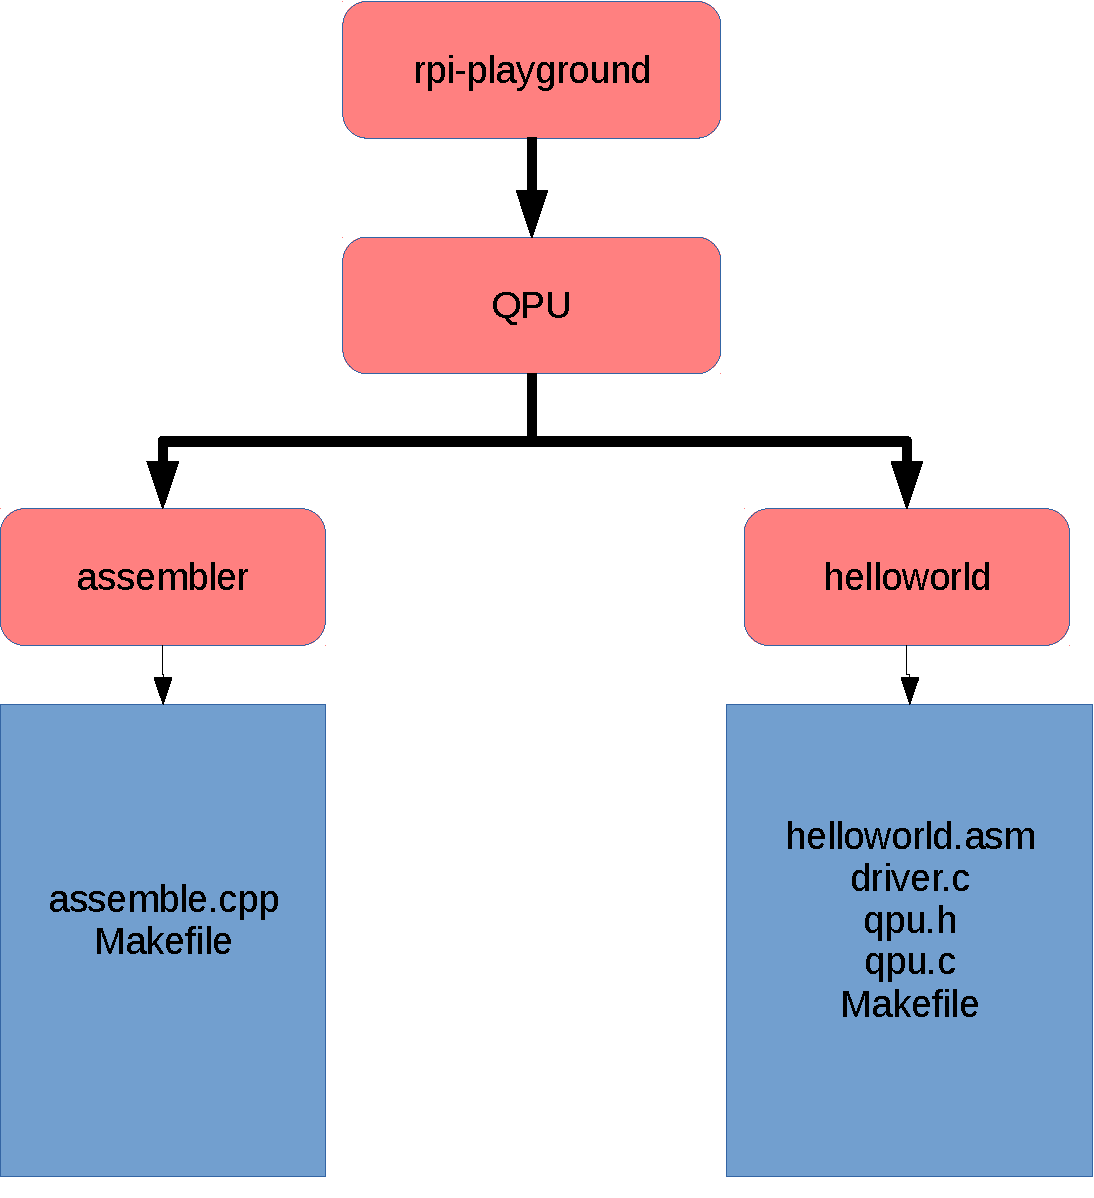
\includegraphics[width=0.4\textwidth,scale=0.2]{rpiPlaygroundArchitecture}
	\caption{\file{rpi-playground} Architecture}
	\label{rpiPlaygroundFigure}
\end{figure}
\FloatBarrier

Figure~\ref{rpiPlaygroundFigure} shows the architecture of the \file{rpi-playground} project once cloned from the \file{github} repository: \code{git clone git@github.com:elorimer/rpi-playground.git}

The project is made of two directories:
\begin{itemize}
\item \keyword{assembler} directory contains:
	\begin{itemize}
		\item \file{assemble.cpp} -- \code{assembly parser} of \vc{} instructions set
	\end{itemize}
\item \keyword{helloworld} directory contains:
	\begin{itemize}
		\item \file{helloworld.asm} -- \code{code-to-execute} on the \vc
		\item \file{driver.c} -- program that \code{drives} the \vc
	\end{itemize}
\end{itemize}


\subsection{assembler directory}


\subsubsection{assemble.cpp}

\file{assemble.cpp} is the \code{assembly parser} written by Eric \textsc{Lorimer}, the author of \file{rpi-playground} project.

This program translates instuctions written in \file{helloworld.asm} - from \file{helloworld} directory figure~\ref{rpiPlaygroundFigure} - into a binary file - \file{helloworld.bin} - that the \vc{} will understand.

Figure~\ref{VCinstructionsFigure} taken from \parencite{refVC} shows the miscellaneous \enquote{\code{add}} operations of the \qpu's instructions set. \vc{} has also \enquote{\code{mul}}, \enquote{\code{load}}, \enquote{\code{branch}} or \enquote{\code{semaphore}} instructions.

\begin{figure}[!htbp]
	\centering
	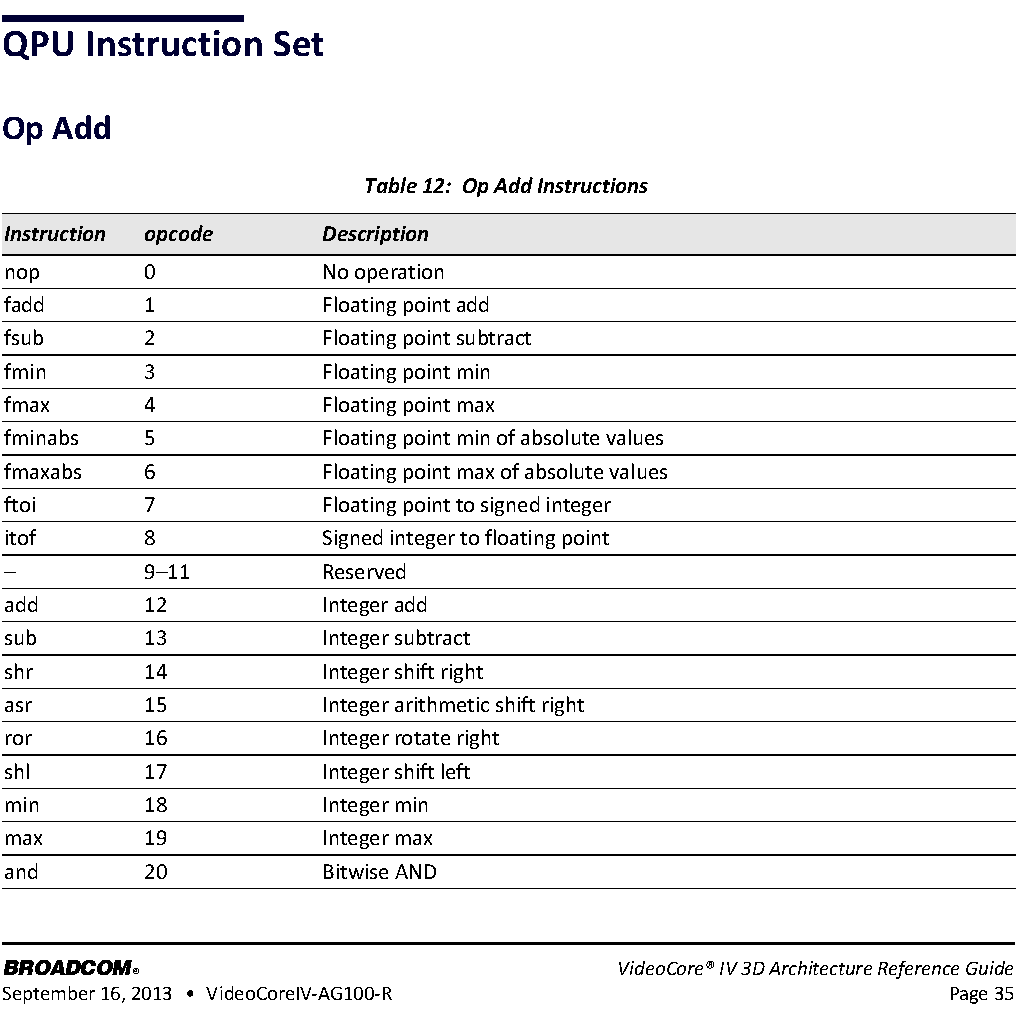
\includegraphics[width=0.6\textwidth]{VCinstructions}
	\caption{Part of \vc{} instructions set}
	\label{VCinstructionsFigure}
\end{figure}
\FloatBarrier
\vspace{5mm}


In \file{assemble.cpp}, these instructions are declared with the following \keyword{C++} code:

\lstset{style=CStyle,caption={Declaration of \code{add} operations in \file{assemble.cpp}},captionpos=t,label=addLabel}
\begin{lstlisting}
static string addOps[] = {
    "nop", "fadd", "fsub", "fmin", "fmax", "fminabs", "fmaxabs",
    "ftoi", "itof", "XXX", "XXX", "XXX", "add", "sub", "shr",
    "asr", "ror", "shl", "min", "max", "and", "or", "xor", "not",
    "clz", "XXX", "XXX", "XXX", "XXX", "XXX", "v8adds", "v8subs" };
\end{lstlisting}


\subsubsection{Makefile}

\lstset{language=make,caption={Makefile from assembler directory},captionpos=t,label=assMakefileLabel}
\begin{lstlisting}
qpu-assembler: assemble.cpp
	g++ -g -o qpu-assembler assemble.cpp
\end{lstlisting}

This \file{Makefile} contains only one instruction. So running the \code{make} command inside the \keyword{assembler} directory generates an \keyword{executable} file: \file{qpu-assembler}.
\vspace{10mm}

Then, this \keyword{executable} is used in the \file{helloworld} directory to generate \file{helloworld.bin}:
\begin{center}
\code{../assembler/qpu-assembler -o helloworld.bin < helloworld.asm}
\end{center}
\newpage

\subsection{helloworld directory}

\subsubsection{qpu.h/qpu.c}

In these files we define \code{BUS\_TO\_PHYS()}, a \code{MACRO} function to convert \emph{VC CPU Bus Addresses} into \emph{ARM Virtual Addresses} - Appendice~\ref{AppendixB}.

Then we use \code{MACROS} to define the \emph{VC CPU Bus Addresses}'s of \vc{} peripherals.

Finally, we declare \code{gpu\_fft\_get\_host\_info()} to get \rasp{} information.

\lstset{style=CStyle,caption={qpu.h}}
\begin{lstlisting}
#define BUS_TO_PHYS(x) ((x)&~0xC0000000)

#define V3D_L2CACTL (0xC00020>>2)
#define V3D_SLCACTL (0xC00024>>2)
#define V3D_SRQPC   (0xC00430>>2)
#define V3D_SRQUA   (0xC00434>>2)
#define V3D_SRQCS   (0xC0043c>>2)
#define V3D_DBCFG   (0xC00e00>>2)
#define V3D_DBQITE  (0xC00e2c>>2)
#define V3D_DBQITC  (0xC00e30>>2)

int gpu_fft_get_host_info(struct GPU_FFT_HOST *info);
\end{lstlisting}


\subsubsection{helloworld.asm}

\file{helloworld.asm} is the \code{code-to-execute} by the \vc. It is written in \option{assembly language} using the \vc{}'s instructions set. Let's explain this \file{file} line by line:\\

\code{\# Load the value we want to add to the input into a register\\ldi ra1, 0x1234}\\
-- First, we load the 32-bit immediate value \emph{0x1234} into \emph{ra1} register.\\
-- This value is replicated 16 ways accross the entire SIMD array of the \emph{QPU 0,0} processor.\\

\code{\# Configure the VPM for writing\\ldi rb49, 0xa0}\\
-- \qpu{} register address map in \parencite{refVC} pages 37-38 shows writting to \emph{rb49} is \code{VPMVCD\_WR\_SETUP}: we configure \keyword{VPM} memory to store results from \emph{QPU 0,0}.\\

\code{\# Add the input value (first uniform - rb32)\\ \# and the register with the hard-coded constant into the VPM.\\add rb48, ra1, rb32; nop}\\
-- \emph{rb48} is the register to write into, in order to write results from the \emph{QPU 0,0} to the \keyword{VPM} the way we just configured it.\\
-- \emph{rb32/ra32} is the address we read from to fetch \keyword{100} -- \keyword{uniform} value.\\

\newpage
\code{\# Move 16 words (1 vector) back to the host (DMA)\\ldi rb49, 0x88010000}\\
-- From \parencite{refVC} page 58, we configure the \emph{VPM DMA storing} by writing \emph{rb49} register : \code{VPMVCD\_WR\_SETUP}.\\
-- We configure the \emph{DMA} transfer of 16-word vector from \emph{VPM buffer} to the \ram{} memory.\\

\code{\# Initiate the DMA (next uniform, ra32, is the host address to write to)\\or rb50, ra32, 0; nop}\\
\code{\# Wait for the DMA to complete\\or rb39, rb50, ra39; nop}\\
-- Finally, we write the results in the \ram{} memory at the second uniforms address \emph{ra32} register.\\

\code{\# Trigger a host interrupt (writing rb38) to stop the program\\or rb38, ra39, ra39; nop}\\
\code{nop.tend ra39, ra39, ra39; nop rb39, rb39, rb39\\nop ra39, ra39, ra39; nop rb39, rb39, rb39\\nop ra39, ra39, ra39; nop rb39, rb39, rb39}\\
-- The last instructions stops the program.


\subsubsection{driver.c}\label{helloworldlabel}

The whole \file{driver.c} program is written in Appendice~\ref{AppendixE}. Here I detail the \keyword{key parts}:

\code{\#include ``mailbox.h''}\\
-- We use the \mail{} interface to communicate between \vc{} and \cpu.\\
-- This interface uses low-level linux kernel functions that enable \keyword{CPU} to send \code{code-to-execute} and \code{input data} called \uni{}s to \keyword{GPU}, and then get back \code{results} from \keyword{GPU}.\\


\lstset{style=CStyle,caption={helloworld memory\_map}, label=map}
\begin{lstlisting}
struct memory_map {
    unsigned int code[MAX_CODE_SIZE];
    unsigned int uniforms[NUM_QPUS][2];
    unsigned int msg[NUM_QPUS][2];
    unsigned int results[NUM_QPUS][16];
};
int code_words = loadShaderCode(argv[1], qpu_code, MAX_CODE_SIZE);
\end{lstlisting}
-- This defines the memory layout we’ll use and share between \keyword{CPU} and \keyword{GPU}.\\
-- This layout will be accessed in both \emph{ARM Virtual Addresses} and \emph{VC CPU Bus Addresses} - Appencice~\ref{AppendixB}.\\
-- We use \code{loadShaderCode()} function to load \file{helloworld.bin} in the \ram. This is the binary file containing the \code{code-to-execute}.
\newpage


\lstset{style=CStyle,caption={initialize \mail{} interface}, label=init}
\begin{lstlisting}
    int mb = mbox_open();
    if (qpu_enable(mb, 1))
    {
        fprintf(stderr, "QPU enable failed.\n");
        return -1;
    }
    printf("QPU enabled.\n");

    unsigned size = 1024 * 1024;
    unsigned handle = mem_alloc(mb, size, 4096, host.mem_flg);
    if (!handle)
    {
        fprintf(stderr, "Unable to allocate %d bytes of GPU memory", size);
        return -2;
    }

    unsigned ptr = mem_lock(mb, handle);
    void *arm\_ptr = mapmem(BUS\_TO\_PHYS(ptr + host.mem\_map), size);
\end{lstlisting}
-- We initialize the \mail{} interface and send a message to enable the \qpu{} with \code{qpu\_enable()} \mail{} function\\
-- We allocate and lock GPU memory with \code{mem\_alloc()} and \code{mem\_lock()} \mail{} functions:
\begin{itemize}
	\item \emph{ptr} is now the base Bus Address of the GPU memory mapping
	\item \emph{ptr} is a \emph{VC CPU BUS Addresses} - Appendice~\ref{AppendixB}
\end{itemize}
-- Last line is a \keyword{key step} in our driver. Keep in mind that \vc{} is an \cpu{} peripheral so, to bind both \emph{VC CPU BUS Addresses} and \emph{ARM Virtual Addresses} we use both \code{mapmem() \& BUS\_TO\_PHYS()} functions.\\
-- Now we have two addresses - Appendice~\ref{AppendixB} - to refer to the memory:
\begin{itemize}
	\item \emph{ptr} is the address that the \vc{} understands in \emph{VC CPU Bus Addresses}. \keyword{When passing pointers from CPU to GPU  we need to use \enquote{ptr}}.
	\item \emph{arm\_ptr} is used when accessing \cpu{} memory in \emph{ARM Virtual Addresses}. \keyword{\enquote{arm\_map} the address that CPU understands}.
\end{itemize}
-- \keyword{Physically, \emph{ptr} and \emph{arm\_ptr} point on the same RAM space}.
\vspace{5mm}


\lstset{style=CStyle,caption={pointer arithmetic},label=arithmetic}
\begin{lstlisting}
    // assert arm_ptr ...
    struct memory_map *arm_map = (struct memory_map *)arm_ptr;
    memset(arm_map, 0x0, sizeof(struct memory_map));

    unsigned vc_uniforms = ptr + offsetof(struct memory_map, uniforms);
    unsigned vc_code = ptr + offsetof(struct memory_map, code);
    unsigned vc_msg = ptr + offsetof(struct memory_map, msg);
    unsigned vc_results = ptr + offsetof(struct memory_map, results);
    memcpy(arm_map->code, qpu_code, code_words * sizeof(unsigned int));
\end{lstlisting}
-- We make pointer arithmetic to bind the same memory layout as \code{memory\_map} - Listing~\ref{map} -  within \emph{VC CPU Bus Addresses} \\
-- Finally we copy \code{code} in memory with \code{memcpy()}. \code{code} is actually \code{helloworld.bin}.
-- So this \code{helloworld.bin} will be accessible by \keyword{GPU} using \emph{VC CPU BUS Addresses}: \code{vc\_code}.
\newpage


\lstset{style=CStyle,caption={Copy uniforms and transfer pointers with execute\_qpu()},label=transfer}
\begin{lstlisting}
    for (int i = 0; i < NUM_QPUS; i++)
    {
        arm_map->uniforms[i][0] = uniform_val;
        arm_map->uniforms[i][1] = vc_results + i * sizeof(unsigned) * 16;
        arm_map->msg[i][0] = vc_uniforms + i * sizeof(unsigned) * 2;
        arm_map->msg[i][1] = vc_code;
    }

    unsigned ret = execute_qpu(mb, NUM_QPUS, vc_msg, GPU_FFT_NO_FLUSH,
                               GPU_FFT_TIMEOUT);
\end{lstlisting}
-- To execute a \qpu{} program on the \keyword{GPU}, we pass an array of message structures \emph{vc\_msg}, through \code{execute\_qpu()} \mail{} function. This array contains:
\begin{itemize}
	\item First - \emph{vc\_uniforms} - a pointer to all the \uni{}s to bind to the QPU program:
	\begin{itemize}
		\item \emph{uniform\_val} - 100
		\item \emph{vc\_results} - address of \code{results[NUM\_QPU][16]} in \emph{VC CPU Bus Addresses}
	\end{itemize}
\item Then - \emph{vc\_code} - a pointer to the address of the \code{code-to-execute} on QPU.
\end{itemize}


\subsection{Summary}

\begin{figure}[!htbp]
	\centering
	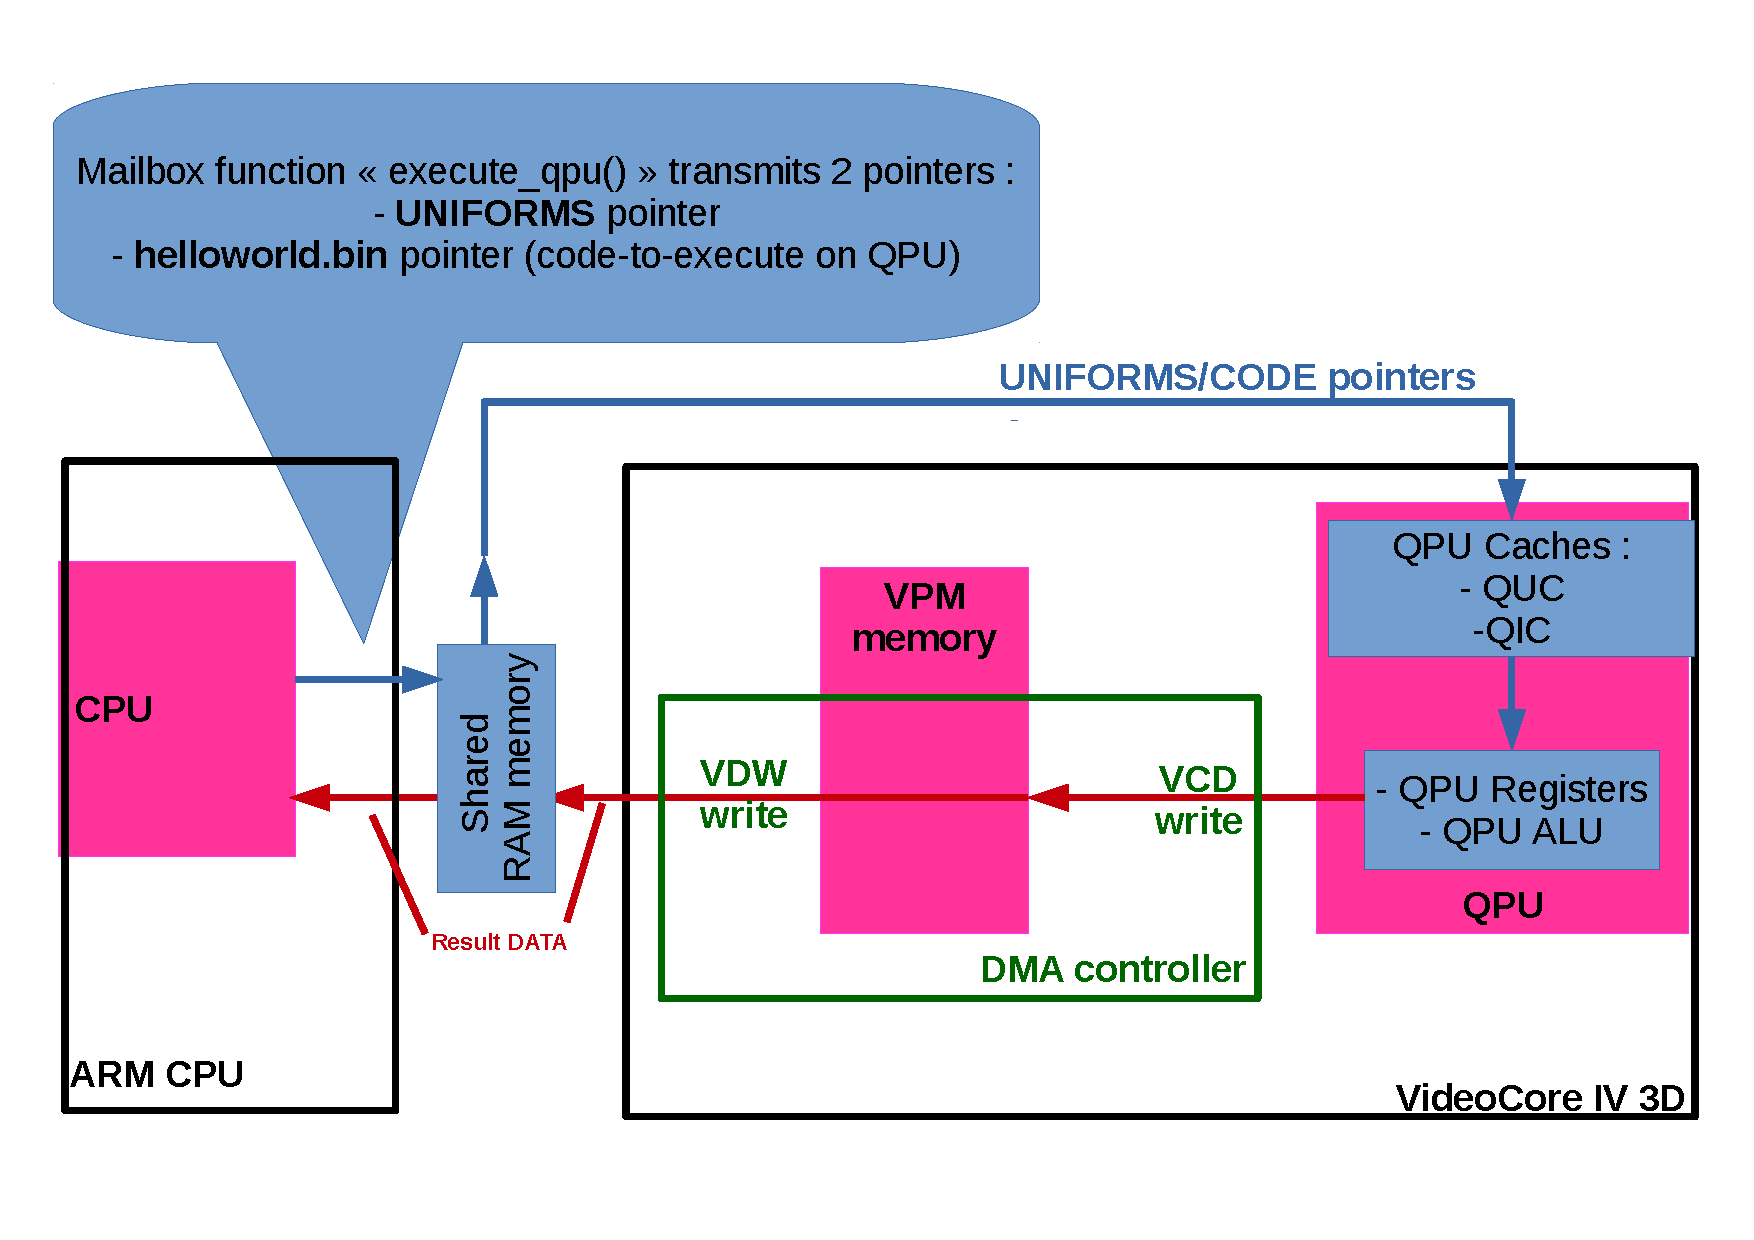
\includegraphics[width=0.9\textwidth]{helloworldDataFlow}
	\caption{\file{helloworld} execution diagram}
	\label{flowFigure}
\end{figure}
\FloatBarrier


Figure~\ref{flowFigure} sums up the \file{helloworld} program execution:

\begin{itemize}
	\item We use two \uni{}s to transfer an \emph{input value} (100) and a pointer to \emph{results array address} - \code{results[NUM\_QPUS][16]} - from the host \cpu{} to the \emph{QPU 0,0}
	\item We send them with \code{execute\_qpu()}, a \mail{} function.
	\item These 2 uniforms will be load into \emph{QUC : Uniforms Cache}.
	\item We also tranfer a pointer to the \code{code-to-execute} on \keyword{GPU}.
	\item \code{code-to-execute} is then load into \emph{QIC : Icache (Instructions cache)}.
	\item \emph{QPU 0,0} adds \emph{100} to \emph{0x1234}.
	\item First, the result (16-word vector) is write back to \keyword{VPM}.
	\item Then, the result (16-word vector) is write back from \keyword{VPM} to \ram{} memory through \keyword{DMA} transfer.
\end{itemize}


\subsection{Conclusion}\label{GPUconclusion}

This project taught me the basis of \vc{} programming and laid the groundwork for the rest of my internship. I understood that:
\begin{itemize}
	\item GPU and CPU share the same RAM memory - Appendice~\ref{AppendixB}
		\begin{itemize}
			\item CPU sends code \keyword{pointers} and variables called \uni{}s in the \emph{VC CPU Bus Addresses}
			\item GPU gives back results in \emph{VC CPU Bus Addresses}
			\item CPU gets results since \emph{ARM Virtual Addresses} and \emph{VC CPU Bus Addresses} are bind together with \code{mapmem()}
		\end{itemize}
	\item GPU is driven by CPU program (\file{driver.c}) that:
		\begin{itemize}
			\item initialize GPU
			\item map \ram{} memory and bind \emph{ARM Virtual Addresses} \& \emph{VC CPU Bus Addresses}
			\item copy code and data in the \ram
			\item send code pointers and variables called \uni{}s in the \emph{VC CPU Bus Addresses}
			\item get back results
		\end{itemize}
	\item GPU and CPU communicate via \mail{}:
		\begin{itemize}
			\item \api{} that uses low-level linux kernel functions
			\item source code is available in the raspbian distribution
		\end{itemize}
	\item GPU processor is called \qpu{} -- Appendice~\ref{AppendixD}:
		\begin{itemize}
			\item SIMD processors -- operates on 16-words vector
			\item 12 QPUs on \vc
		\end{itemize}
	\item GPU is fitted with - Appendice~\ref{AppendixC}:
		\begin{itemize}
			\item VPM to store result from QPU
			\item DMA to send result from VPM to \ram{} memory
		\end{itemize}
	\item To run program on GPU:
		\begin{itemize}
			\item \code{code-to-execute} is written in \keyword{assembly language} - \file{helloworld.asm}
			\item \code{code-to-execute} is translate into \keyword{binary} file - \file{helloworld.bin}
			\item \code{code-to-execute} is copied in \ram{} by the \cpu
			\item \code{code-to-execute} pointer is sent to \keyword{GPU}
			\item \code{variables} called \uni{}s are sent to \qpu{}
			\item \vc{} gives back in the \emph{VC CPU Bus Addresses}
		\end{itemize}
\end{itemize}
To build the homemade \api{} for \iBubble, I focused on:
\begin{itemize}
	\item improve \file{driver.c}
	\item refactore project architecture
	\item use a more comprehensive \code{assembly parser} than \file{assemble.cpp}
	\item find new \vc{} features
	\item include my source code in \keyword{C++} project
\end{itemize}

%----------------------------------------------------------------------------------------

\section{Standard Project}

\subsection{\emph{pi-gemm} Project}

\emph{pi-gemm} \parencite{refPiGemm} is a project written by Pete \textsc{Warden} with associated \file{github}: \url{https://github.com/jetpacapp/pi-gemm}. It implements optimized \emph{GEMM} algorithm on \vc.

This project is interesting for several reasons:
\begin{itemize}
	\item the author wrote an improved \code{assembly parser} -- \file{qpu-asm.cpp}
	\item \emph{pi-gemm} introduces the \keyword{TMU} -- Appendice~\ref{AppendixC}
	\item multiply matrix is massively used in \flow{} processing
	\item \emph{pi-gemm} algorithm is called in a \file{main.cpp} file -- as our homemade \api
	\item \emph{pi-gemm} \file{Makefile} is more generic
\end{itemize}


\subsection{Texture Memory Unit and Matrices}\label{Matrices}

\emph{pi-gemm} introduces the way to use matrices and \keyword{TMU}, a new crucial component of \vc{}.

\keyword{TMU} enables \qpu{} to directly access data from the \ram{}. We just have to pass data pointer from the \emph{VC CPU Bus Addresses} in some \keyword{uniforms} variables to load the values containing at this address.

For instance, matrices which are stored in the \ram{} can be accessed knowing the pointer of the first element. I also noticed that matrices are stored in \emph{row-major} order (Figure~\ref{rowcolumnarrays}). That means row values are contiguous in \ram{} memory. This is a \keyword{key point} to know because frames from the \rasp{} camera are stored as \option{float-matrices} in memory and to compute the \flow{} we have to access data from those frames.

\begin{figure}[!htbp]
	\centering
	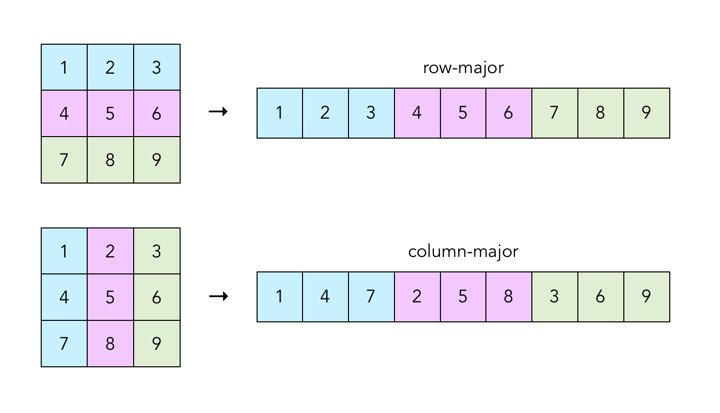
\includegraphics[width=0.6\textwidth]{rowcolumnarrays}
	\caption{Row-major vs. Colon-major matrices}
	\label{rowcolumnarrays}
\end{figure}
\FloatBarrier


\subsection{Refactoring projects}

My goal while studying \emph{pi-gemm} project was to create a standard framework to develop my own projects. I finally came with a mix between both \file{helloworld} and \file{pi-gemm} projects. Figure~\ref{projectArchitectureFigure} shows my project architecture:

\begin{figure}[!htbp]
	\centering
	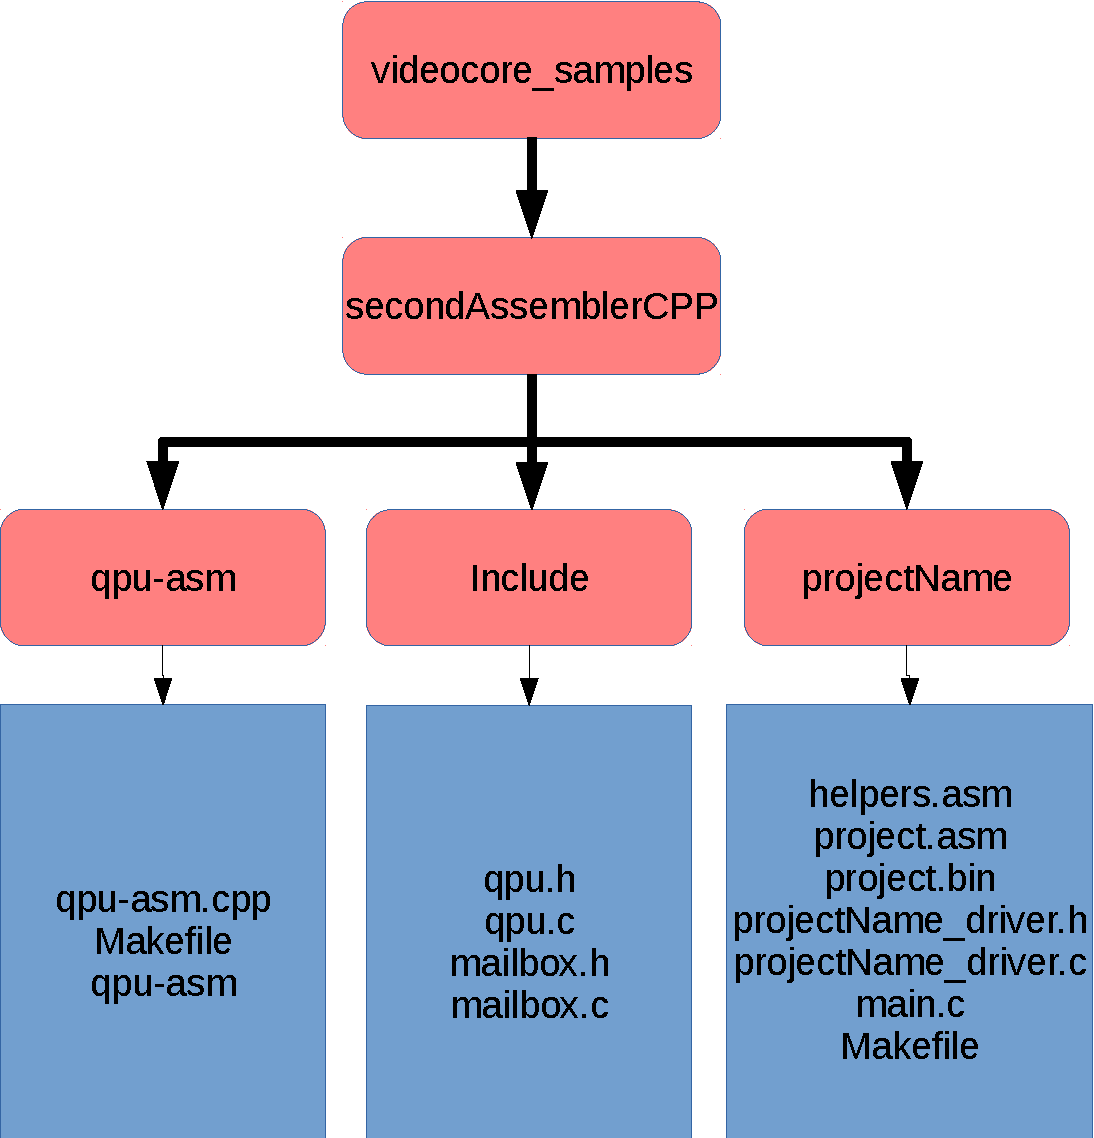
\includegraphics[width=0.4\textwidth,scale=0.2]{projectArchitecture}
	\caption{Standard Framework Project Architecture}
	\label{projectArchitectureFigure}
\end{figure}
\FloatBarrier


\subsubsection{qpu-asm}

This directory contains 3 files: \file{qpu-asm.cpp}, \file{Makefile}, and \file{qpu-asm}.

\file{qpu-asm.cpp} is the \code{assembly parser} from \file{pi-gemm} written by Pete \textsc{Warden}. It is more comprhensive because it features more instructions of the \vc.

\lstset{language=make,caption={},captionpos=t,label=}
\begin{lstlisting}
qpu-assembler: assemble.cpp
	g++ -g -o qpu-assembler assemble.cpp
\end{lstlisting}

Run the \code{make} command will generate \file{qpu-asm}, an \keyword{executable} file and then:\\
\begin{center}
\code{./qpu-asm -o projectName.bin < projectName.asm}
\end{center}


\subsubsection{Include}

This directory contains 4 files: \file{qpu.h}, \file{qpu.c}, \file{mailbox.h} and \file{mailbox.c}.
Those files are included into the \emph{Raspbian Stretch Lite} distribution and allow us to use the \mail{} interface to communicate between \vc{} and \cpu.

I included \mail{} source code directly in this directory for more software portabilty.

\subsubsection{projectName}

\file{projectName} directory contains:
\begin{itemize}
	\item \file{project.asm}/\file{project.bin} -- \code{code-to-execute} on \vc.
	\item \file{projectName\_driver.h}/\file{projectName\_driver.c} -- \keyword{GPU} driver that contains functions to map memory, send data and code to \vc{} etc \ldots
	\item \file{main.c} -- invoke functions from \file{projectName\_driver.c} to run \code{code-to-execute} on \vc.
	\item \file{Makefile} -- generic \file{Makefile} that generates an \keyword{executable} called \file{projectName} - Appendice~\ref{AppendixF}.
\end{itemize}


\subsubsection{Run project}
\lstset{language=make,caption={},captionpos=t,label=}
\begin{lstlisting}
cd qpu-asm
make qpu-asm
cd projectName
make
sudo ./projectName
\end{lstlisting}


\subsubsection{Project Examples}

Once this standard framework was running well, I started developping several projects to run on the \rasp. The goal was to learn more \vc{}'s features and architecture. For instance I developped programs that:
\begin{itemize}
	\item take two 16-word vectors from \cpu{} memory, copy and multiply them inside \ram{} and give back result to \cpu
	\item take a $(240\times 360)float-matrix$ from \cpu{} memory, copy it inside \ram{}, convoluate it by a $(3\times 3)kernel$ and give back the resulting $(238\times 358)float-matrix$ to \cpu
\end{itemize}
\newpage

%----------------------------------------------------------------------------------------

\section{Miscellaneous achievements}

In addition to my research on \vc{}'s projects, I developped several other helpful skills in software development during this internship.


\subsection{Linux \& Vim}

At \groupname{} the software developpment is done using GNU/Linux OS. Thus I used \emph{GCC} or \emph{G++} compilers and I got immersed in Linux Architecture, Command Line or in Makefile writting. I also needed to compile some libraries (\emph{Python, OpenCV} from scratch and face some compiling error after hours of running.

Since I developped on \rasp{}, I started using \emph{Vim} editor. Nicolas \textsc{Vincent} a member of the embedded software team, conviced me to start using this very \emph{customizable} editor. He learned me the basis and how to add useful plug-ins. He was a great adviser for me and taught me a lot of tricks.


\subsection{git \& github}

Another very helpful skill I gained during my internship is in \emph{git} and \emph{github} using. I started to use \code{git clone} to copy projects on my \rasp.

Within \groupname{} I created my first professional \emph{repository} called \keyword{videocore\_samples}: \url{https://github.com/notiloPlus/videocore_samples}. In this repository I put all the projects I developped to explore the \vc.

I made this repository very teaching in order to learn other people how to use \vc. To do that, I wrote my \emph{README.md} file to explain how to use this repository. I had to learn how to write \file{markdown(.md)} files.

I maintained this repository using \code{git add}, \code{git commit} and \code{git push} commands.


\subsection{\LaTeX}

When came time to write this report I decided to use \LaTeX{}. I found a template that I customized to fill my needs. I didn't use any IDE but I added a \LaTeX{} plug-in to \emph{Vim} to continue learning how to use this editor. It was my first major report written in \LaTeX{} so the beginning was harsh. Nevertheless, I finished without any compiling errors and the result is very stylish.

%----------------------------------------------------------------------------------------

\section{Conclusion}\label{Conclusion2}

At the end of this internship work, I was more confortable to deal with my internship subject. So I started developping the \api{} to use \vc. I had more interactions with Camille to build the \flow{} project.
